\chapter{Eredmények} \label{resultsChapter}

A méréseket az alábbi paraméterekkel rendelkező számítógépen végeztem:
\begin{itemize}
	\item	CPU: 11th Gen Intel(R) Core(TM) i5-11300H @ 3.10GHz
	\item	GPU: NVIDIA GeForce RTX 3050Ti 
	\item	RAM: 24 GB DDR4 
	\item	OS: Windows 10 Education 22H2 
	\item	Compiler: NVCC V12.0.140
	
\end{itemize}

\section{A mérések menete}
Az algoritmusokhoz készítettem CPU és GPU kódot is. Az algoritmusok érdemi részét végig GPU-n végeztem. CPU-n a kezdeti értékeket állítottam be, különböző diagnosztikai kiíratásokat végeztem, illetve a parancssori argumentumok feldolgozását. A futásidők méréséhez az NVIDIA által készített Nsight Compute(R) programot használtam, mely képes CUDA kerneleket elemezni több szempontból is: Futási idő, Memória kihasználtsága, Grid mérete, szálanként regiszterek száma és még tovább. A program futását \ref{fig:nsight-compute}. ábrán ábrázoltam. 

\begin{figure}[ht!]
	\centering
	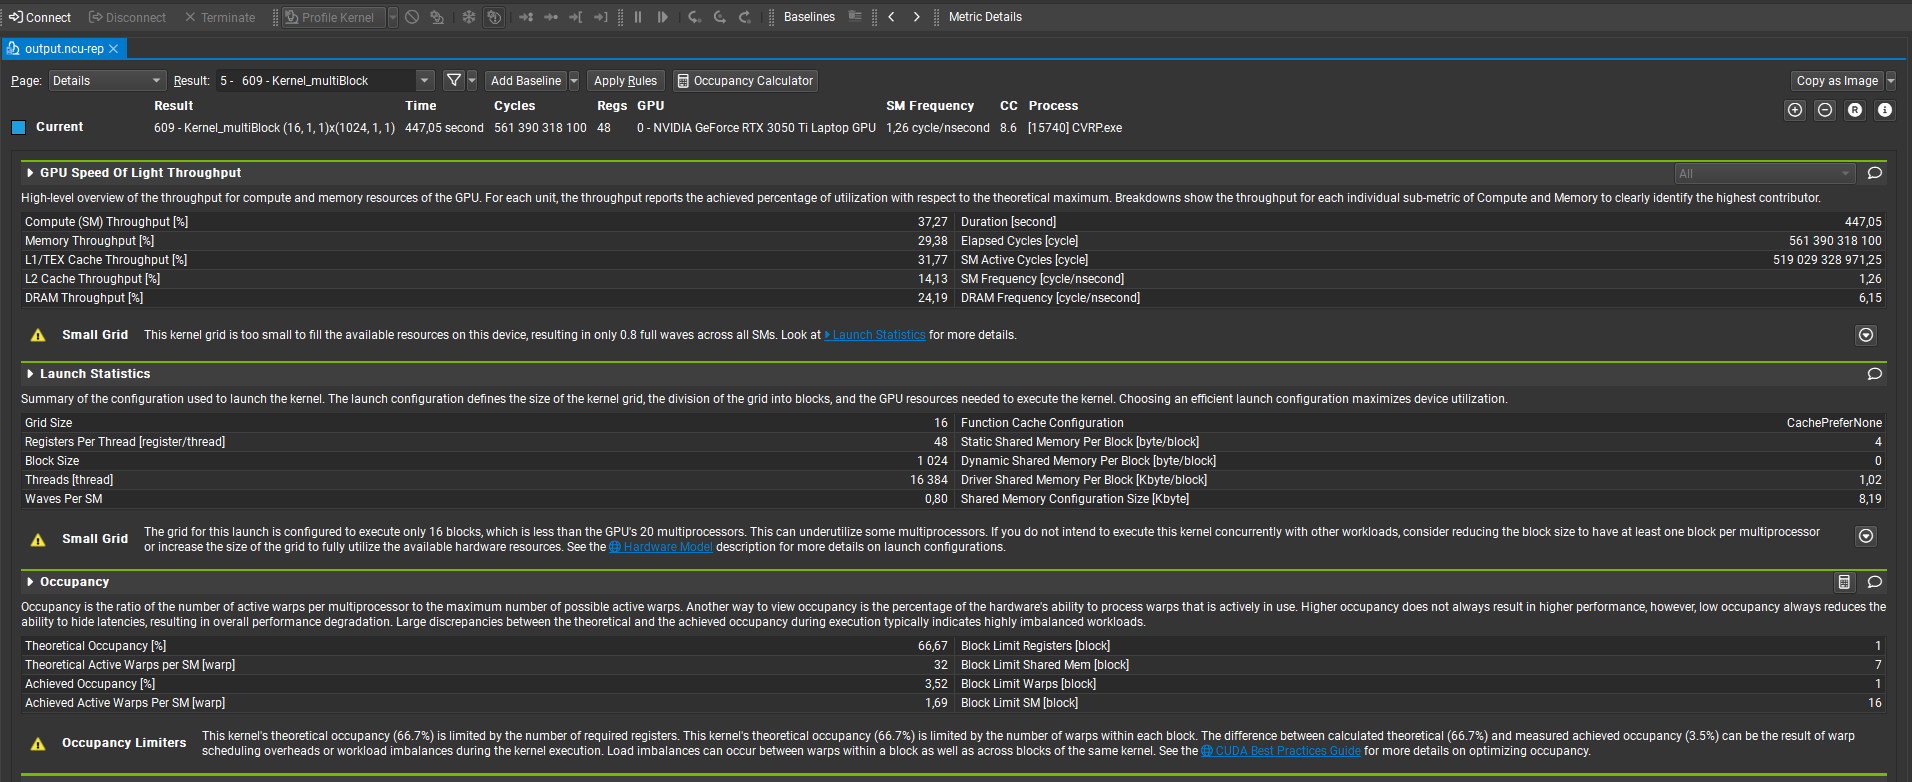
\includegraphics[width=150mm, keepaspectratio]{figures/nsight-compute.png}
	\caption{Az NVIDIA Nsight Compute program adatok széles tárházával látja el a programozót }
	\label{fig:nsight-compute}
\end{figure}

%TODO Konfigról a képet már csak be kell tenni

Számomra a legfontosabb a futásidő volt, ezt több különböző bemenetre és konfigurációra lemértem, majd táblázatosan összegyűjtöttem.

\section{Mérési eredmények}

A továbbiakban táblázatokba szedtem az egyes algoritmusokon végzett profilozó méréseim eredményeit. A futásidők időegysége másodperc, mert ilyen nagyságrendben mozogtak az értékek. Többször lefuttattam a programokat ugyanolyan paraméterek mellett, ebből lejegyeztem az átlagos eredményeket (10 futás számtani közepe) és a legkisebb kapott megoldást.

\subsection{TSP első verzió}

Teszteléshez szükségem volt ismert eredményű adathalmazokra. A Floridai Állami Egyetem weboldalán \cite{TSPdataset} elérhető bárki számára több adathalmaz, különböző adatstruktúrában. Nekem a [fájlnév]\_d.txt nevű fájlok voltak hasznosak, ugyanis abban megtalálhatóak a szomszédossági mátrix költségei táblázatos alakban. Az itt található 6 adathalmazon végigfuttattam az algoritmusomat több konfigurációban. Mindig 10-szer ismételtem meg a futást, és képeztem az eredmények átlagát (számtani középpel), illetve minimumát. Nagy adathalmaz esetén hosszú a futásidő profilozó módban, ezért időmérés céljából egyszer futtattam újra ugyanazon beállításokkal. A TSP első verziójában a feromon mátrix és az élsúlyok tárolása csak double formátumban történik. Az összehasonlíthatóság érdekében egy iteráció során 20 random, és 500 tudatos hangya fut. A kezdeti feromon érték 1000, az elnyomási tényező \( \rho = 0.75 \), a jutalmazási arány 100, amely csak a 2. iterációtól érvényes (ha van).



% Size = 5
\begin{table}[ht!]
	\centering
	\begin{tabular}{|p{2cm}||p{3cm}|p{3.5cm}|p{3.5cm}|}
		\hline
		\multicolumn{4}{|c|}{FIVE : 5 csúcs, minimális út : 19, átlagos út : 24} \\
		\hline
		& Futásidő (ms) & Végeredmény átlag & Végeredmény min.\\
		\hline
		\textbf{1 rep} & & &\\
		32 ant& 7,84 & 20,2 & 19\\
		256 ant & 19,1 & 20,8 & 19\\
		1024 ant & 76,1 &	20,8 &	19\\
		\hline
		\textbf{10 rep} & & &\\
		256 ant & 137,3 & 19 &	19\\
		1024 ant & 424 &	19 &	19\\
		\hline
	\end{tabular}
	\caption{Elsőnek egy kicsi, 4 állomásból (és a 0. kiindulási pontból) álló gráfon próbáltam ki az algoritmust.}
	\label{table:TSPv1_5}
\end{table}

% Size = 15
\begin{table}[ht!]
	\centering
	\begin{tabular}{|p{2cm}||p{3cm}|p{3.5cm}|p{3.5cm}|}
		\hline
		\multicolumn{4}{|c|}{P01 : 15 csúcs, minimális út : 291, átlagos út : 662} \\
		\hline
		& Futásidő (s) & Végeredmény átlag & Végeredmény min.\\
		\hline
		\textbf{1 rep} & & &\\
		1024 ant & 0,925 & 370,2 & 291\\
		2048 ant & 1,18 & 365 & 327\\
		4096 ant & 1,20 & 359,7 & 332\\
		\hline
		\textbf{10 rep} & & &\\
		1024 ant & 11,39 & 350,4 & 291\\
		2048 ant & 11,47 & 328 & 295\\
		4096 ant & 11,59 & 336,8 & 291\\
		\hline
	\end{tabular}
	\caption{}
	\label{table:TSPv1_15}
\end{table}

A 17 vagy nála nagyobb gráfok esetében az 1 iterációs algoritmusok már olyan rosszul teljesítettek, hogy csak 10 iterációs eseteket soroltam fel a hangyák számának függvényében.

% Size = 17
\begin{table}[ht!]
	\centering
	\begin{tabular}{|p{2cm}||p{3cm}|p{3.5cm}|p{3.5cm}|}
		\hline
		\multicolumn{4}{|c|}{GR : 17 csúcs, minimális út : 2085} \\
		\hline
		& Futásidő (s) & Végeredmény átlag & Végeredmény min.\\
		\hline
		\textbf{10 rep} & & & \\
		1024 ant & 14,85 & 2391,3 & 2151\\
		2048 ant & 14,88 & 2363,4 & 2085\\
		4096 ant & 14,97 & 2279,6 & 2097\\
		8192 ant & 15,15 & 2306,4 & 2207\\
		16384 ant & 15,49 & 2250,5 & 2085\\
		20480 ant & 15,68 & 2221,7 & 2085 \\
		\hline
	\end{tabular}
	\caption{}
	\label{table:TSPv1_17}
\end{table}

% Size = 26
\begin{table}[ht!]
	\centering
	\begin{tabular}{|p{2cm}||p{3cm}|p{3.5cm}|p{3.5cm}|}
		\hline
		\multicolumn{4}{|c|}{FRI26 : 26 csúcs, minimális út : 937, átlagos út : 2693} \\
		\hline
		& Futásidő (s) & Végeredmény átlag & Végeredmény min.\\
		\hline
		\textbf{10 rep} & & & \\
		1024 ant & 39,72 & 1386,1 & 1249\\
		2048 ant & 39,73 & 1367,1 & 1221\\
		4096 ant & 39,82 & 1227,6 & 1121\\
		8192 ant & 40,14 & 1158,7 & 1102\\
		16384 ant & 40,70 & 1132,1 & 1075\\
		20480 ant & 42,72 & 1152,3 & 1097 \\
		\hline
	\end{tabular}
	\caption{}
	\label{table:TSPv1_26}
\end{table}

% Size = 42
\begin{table}[ht!]
	\centering
	\begin{tabular}{|p{2cm}||p{3cm}|p{3.5cm}|p{3.5cm}|}
		\hline
		\multicolumn{4}{|c|}{DANTZIG42 : 42 csúcs, minimális út : 699, átlagos út : 3110,5} \\
		\hline
		& Futásidő (s) & Végeredmény átlag & Végeredmény min.\\
		\hline
		\textbf{10 rep} & & & \\
		1024 ant & 115,41 & 1735,7 & 1554\\
		2048 ant & 113,94 & 1420 & 1252\\
		16384 ant & 114,34 & 987,7 & 906\\
		20480 ant & 113,55 & 931,6 & 879 \\
		\hline
	\end{tabular}
	\caption{}
	\label{table:TSPv1_42}
\end{table}

%%%
%

%%

% Size = 48
\begin{table}[htbp!]
	\centering
	\begin{tabular}{|p{2cm}||p{3cm}|p{3.5cm}|p{3.5cm}|}
		\hline
		\multicolumn{4}{|c|}{ATT48 : 48 csúcs, minimális út : 33523, átlagos út : 157686,9} \\
		\hline
		& Futásidő (s) & Végeredmény átlag & Végeredmény min.\\
		\hline
		\textbf{10 rep} & & & \\
		1024 ant & 156,7 & 79993.2 & 75601 \\
		8192 ant & 152,82 & 56097,9 & 51139 \\
		16384 ant & 153,78 & 50197,2 & 47387 \\
		20480 ant & 154,28 & 46360,8 & 43167 \\
		\hline
	\end{tabular}
	\caption{}
	\label{table:TSPv1_48}
\end{table}



\subsection{TSP második (konzisztens) verzió}
Azért, hogy az előző fejezetben látott első verzióval érdemben össze tudjam hasonlítani a mostani verziót, hasonló iterációs számokat választottam: 1 rep-en belül 20 random hangyát követ 500 tudatos hangya. Az adathalmaz is az előbbi \cite{TSPdataset} helyről származó csomag. A számértékeket összevetve szembetűnő a gyorsulás az előző verzióhoz képest. A legfőbb szerepe ebben úgy gondolom, hogy az adatok double-ről float-ra cserélése, illetve a függvények között szigorú pointer alapú paraméterátadás jelentette.

% Size = 15
\begin{table}[ht!]
	\centering
	\begin{tabular}{|p{2cm}||p{3cm}|p{3.5cm}|p{3.5cm}|}
		\hline
		\multicolumn{4}{|c|}{P01 : 15 csúcs, minimális út : 291, átlagos út : 662} \\
		\hline
		& Futásidő (s) & Végeredmény átlag & Végeredmény min.\\
		\hline
		\textbf{10 rep} & & &\\
		1024 ant & 2,69 & 320  & 307\\
		2048 ant & 2,82 & 307,6 & 291\\
		4096 ant & 2,97 & 305,4 & 291\\
		8192 ant & 3,19 & 300,2 & 291\\
		12288 ant & 3,50 & 296,4 & 291\\
		16384 ant & 3,73 & 294,6 & 291\\
		20480 ant & 3,92 & 295,4 & 291\\
		\hline
		\textbf{30 rep} & & &\\
		1024 ant & 8,05 & 301,6 & 291\\
		20480 ant & 13,37 & 291 & 291\\
		\hline
	\end{tabular}
	\caption{}
	\label{table:TSPv2_15}
\end{table}

% Size = 17
\begin{table}[ht!]
	\centering
	\begin{tabular}{|p{2cm}||p{3cm}|p{3.5cm}|p{3.5cm}|}
		\hline
		\multicolumn{4}{|c|}{GR : 17 csúcs, minimális út : 2085} \\
		\hline
		& Futásidő (s) & Végeredmény átlag & Végeredmény min.\\
		\hline
		\textbf{10 rep} & & & \\
		1024 ant & 3,54 & 2246 & 2094\\
		2048 ant & 3,69 & 2237,7 & 2207\\
		4096 ant & 3,69 & 2196,5 & 2142\\
		8192 ant & 3,89 & 2211,5 & 2170\\
		16384 ant & 4,37 & 2179,2 & 2129\\
		20480 ant & 4,55 & 2175,1 & 2134 \\
		\hline
		\textbf{30 rep} & & & \\
		20480 ant & 13,38 & 2146,5 & 2103 \\
		\hline
	\end{tabular}
	\caption{}
	\label{table:TSPv2_17}
\end{table}

% Size = 26
\begin{table}[ht!]
	\centering
	\begin{tabular}{|p{2cm}||p{3cm}|p{3.5cm}|p{3.5cm}|}
		\hline
		\multicolumn{4}{|c|}{FRI26 : 26 csúcs, minimális út : 937, átlagos út : 2693} \\
		\hline
		& Futásidő (s) & Végeredmény átlag & Végeredmény min.\\
		\hline
		\textbf{10 rep} & & & \\
		1024 ant & 9,00 & 1393 & 1347\\
		2048 ant & 9,23 & 1363,1 & 1288\\
		4096 ant & 9,43 & 1215,3 & 1163\\
		8192 ant & 9,72 & 1136,9 & 1055\\
		16384 ant & 10,82 & 1104,9 & 1007\\
		20480 ant & 11,61 & 1111,7 & 1058 \\
		\hline
		\textbf{30 rep} & & & \\
		20480 ant & 32,93 & 1098,2 & 1047 \\
		\hline
	\end{tabular}
	\caption{}
	\label{table:TSPv2_26}
\end{table}

% Size = 42
\begin{table}[ht!]
	\centering
	\begin{tabular}{|p{2cm}||p{3cm}|p{3.5cm}|p{3.5cm}|}
		\hline
		\multicolumn{4}{|c|}{DANTZIG42 : 42 csúcs, minimális út : 699, átlagos út : 3110,5} \\
		\hline
		& Futásidő (s) & Végeredmény átlag & Végeredmény min.\\
		\hline
		\textbf{10 rep} & & & \\
		1024 ant & 26,19 & 1601,3 & 1018\\
		2048 ant & 26,61 & 1488,4 & 1319\\
		4096 ant & 27,02 & 1286,7 & 1168\\
		8192 ant & 27,57 & 1118,3 & 1004\\
		16384 ant & 31,2 & 1014,7 & 909\\
		20480 ant & 33,31 & 964,9 & 822 \\
		\hline
		\textbf{30 rep} & & & \\
		20480 ant & 99,83 & 972,8 & 886 \\
		\hline
	\end{tabular}
	\caption{}
	\label{table:TSPv2_42}
\end{table}

%TODO: Vízszintes vonalak a repek közé

%%%
%

%%

% Size = 48
\begin{table}[htbp!]
	\centering
	\begin{tabular}{|p{2cm}||p{3cm}|p{3.5cm}|p{3.5cm}|}
		\hline
		\multicolumn{4}{|c|}{ATT48 : 48 csúcs, minimális út : 33523, átlagos út : 157686,9} \\
		\hline
		& Futásidő (s) & Végeredmény átlag & Végeredmény min.\\
		\hline
		\textbf{10 rep} & & & \\
		1024 ant & 38,12 & 84660,7 & 67541 \\
		2048 ant & 38,63 & 72522,8 & 64969 \\
		4096 ant & 39,14 & 62808,6 & 53395 \\
		8192 ant & 39,69 & 59604,8 & 52514 \\
		16384 ant & 41,56 & 48618,2 & 46227 \\
		20480 ant & 41,93 & 49879,9 & 45836\\
		\hline
		\textbf{30 rep} & & & \\
		20480 ant & 124,72 & 47562,9 & 44144 \\
		\hline
	\end{tabular}
	\caption{}
	\label{table:TSPv2_48}
\end{table}


\subsection{VRP}
A VRP-hez eleinte nem értettem, hogy miért nem találtam külön adathalmazt. Később megértettem, hogy mivel nincs megadva egyéb feltétel, (általában) teljesen mindegy, hogy hány járművet használhat az algoritmus, a legjobban akkor fog járni, ha az összes állomást ugyanazon járművel járja végig. A VRP-hez is készült külön kódimplementáció. Ez azért jó, mert amikor különböző feltételeket szabunk meg, elég annyit tenni, hogy az adott feltételt kiértékelő függvényt megírva meghívjuk az eredményt értékelő (antRouteLength) programrészben.


\subsection{CVRP}
Az első olyan algoritmus, amely feltételes útvonaltervezést igényel, a Kapacitásos jármű útvonaltervezési feladat. Adathalmazt a következő helyről szedtem: \cite{CVRPdataset}.
Az iterációk az előzőeknél látottakkal megegyezőek: 1 rep-en belül 20 random hangyát követ 500 tudatos hangya.


% Size = 17
\begin{table}[ht!]
	\centering
	\begin{tabular}{|p{2cm}||p{3cm}|p{3.5cm}|p{3.5cm}|}
		\hline
		\multicolumn{4}{|c|}{17-city problem (Groetschel): 17 csúcs, minimális út: 2685} \\
		\hline
		& Futásidő (s) & Végeredmény átlag & Végeredmény min.\\
		\hline
		\textbf{10 rep} & & & \\
		1024 ant & 2,96 & 3158,7 & 2726  \\
		16384 ant & 3,44 & 2790,4 & 2711 \\
		20480 ant & 3,83 & 2800,5 & 2685 \\
		\hline
		\textbf{30 rep} & & & \\
		1024 ant & 6,05 & 2975,2 & 2685\\
		16384 ant & 10,64 & 2846,2 & 2727 \\
		20480 ant & 13,80 & 2758.5 & 2685 \\
		\hline
		\textbf{50 rep} & & & \\
		1024 ant & 9,97 & 2927,5 & 2685 \\
		16384 ant & 17,64 & 2805,9 & 2685\\
		20480 ant & 18,51 & 2990,1 & 2685\\
		\hline
	\end{tabular}
	\caption{}
	\label{table:CVRP_gr17}
\end{table}

% Size = 21
\begin{table}[ht!]
	\centering
	\begin{tabular}{|p{2cm}||p{3cm}|p{3.5cm}|p{3.5cm}|}
		\hline
		\multicolumn{4}{|c|}{21-city problem (Groetschel): 21 csúcs, minimális út: 3704} \\
		\hline
		& Futásidő (s) & Végeredmény átlag & Végeredmény min.\\
		\hline
		\textbf{10 rep} & & & \\
		1024 ant & 2,96 & 5026,3 & 4389 \\
		16384 ant & 4,75 & 4217 & 4068 \\
		20480 ant & 5,72 & 4103,3 & 3903 \\
		\hline
		\textbf{30 rep} & & & \\
		1024 ant & 8,31 & 4770,5 & 4001 \\
		16384 ant & 12,17 & 4105,4 & 3864 \\
		20480 ant & 16,61 & 4133 & 3881\\
		\hline
		\textbf{50 rep} & & & \\
		1024 ant & 19,76 & 4467,5 & 3758 \\
		16384 ant & 22,73 & 4259,3 & 4090 \\
		20480 ant & 28,03 & 4211,6 & 4053 \\
		\hline
	\end{tabular}
	\caption{}
	\label{table:CVRP_gr21}
\end{table}

% Size = 33
\begin{table}[ht!]
	\centering
	\begin{tabular}{|p{2cm}||p{3cm}|p{3.5cm}|p{3.5cm}|}
		\hline
		\multicolumn{4}{|c|}{Augerat et al: 33 csúcs, minimális út: 742} \\
		\hline
		& Futásidő (s) & Végeredmény átlag & Végeredmény min.\\
		\hline
		\textbf{10 rep} & & &\\
		1024 ant & 5,62 & 1571,62 & 1283,05 \\
		16384 ant & 8,61 & 1496,24 & 1342,16 \\
		20480 ant & 13,01 & 1470,99 (+98.25\%) & 1310,18 (+76.57\%) \\
		\hline
		\textbf{30 rep} & & & \\
		1024 ant & 22,74 & 1529,4 & 1351,81 \\
		16384 ant & 23,68 & 1375,43 & 1209,97 \\
		20480 ant & 35,24 & 1415,17 (+90.72\%) & 1182,57 (+59.38\%) \\
		\hline
		\textbf{50 rep} & & & \\
		1024 ant & 24,91 & 1434,34 & 1230\\
		16384 ant & 41,26 & 1421,19 & 1361,51 \\
		20480 ant & 61,01 & 1402,18 (+88.97\%) & 1092,92 (+47.29\%) \\
		\hline
	\end{tabular}
	\caption{}
	\label{table:CVRP_a33}
\end{table}

% Size = 48
\begin{table}[ht!]
	\centering
	\begin{tabular}{|p{2cm}||p{3cm}|p{3.5cm}|p{3.5cm}|}
		\hline
		\multicolumn{4}{|c|}{Rinaldi,Yarrow/Araque: 48 csúcs, minimális út: 40002} \\
		\hline
		& Futásidő (s) & Végeredmény átlag & Végeredmény min.\\
		\hline
		\textbf{10 rep} & & & \\
		1024 ant & 44,28 & 89736,85 (+124\%) & 56813,06 (+42\%) \\
		16384 ant & 44,86 & 83208,23 (+108\%) & 57162,13 (+43\%) \\
		20480 ant & 48,89 & 89271,67 (+123\%) & 56966,07 (+42\%) \\
		\hline
		\textbf{30 rep} & & & \\
		1024 ant & 76,93 & 81507,64 & 67745 \\
		16384 ant & 133,62 & 74530,89 (+86.32\%) & 58940,59 (+47.34\%) \\
		20480 ant & 146,36 & 76197,09 (+90.48\%) & 53783,10 (+34.45\%) \\
		\hline
		\textbf{50 rep} & & & \\
		1024 ant & 223,39 & 75265,07 (+88.15\%) & 58007,69 (+45.01\%) \\
		16384 ant & 223,5 & 69196,02 (+72.98\%) & 54812,73 (+37.02\%) \\
		20480 ant & 215,03 & 64510,92 (+61.27\%) & 56817,40 (+42.04\%) \\
		\hline
	\end{tabular}
	\caption{}
	\label{table:CVRP_att48}
\end{table}

% Size = 72
\begin{table}[ht!]
	\centering
	\begin{tabular}{|p{2cm}||p{3cm}|p{3.5cm}|p{3.5cm}|}
		\hline
		\multicolumn{4}{|c|}{Fisher problem 11: 72 csúcs, minimális út: 237} \\
		\hline
		& Futásidő (s) & Végeredmény átlag & Végeredmény min.\\
		\hline
		\textbf{10 rep} & & & \\
		16384 ant & 110,84 & 887,96 & 645,34\\
		20480 ant & 112,34 & 923,91 (+289.84\%) & 874,96 (+269.18\%)\\
		\hline
		\textbf{30 rep} & & & \\
		16384 ant & 292,38 & 764,31 & 551,81 \\
		20480 ant & 346,49 & 706,20 (+197.97\%) & 458,31 (+93.38\%) \\
		\hline
		\textbf{50 rep} & & & \\
		16384 ant & 478,71 & 732,96 (+209.27\%) & 574,85 (+142.55\%)\\
		20480 ant & 572,36 & 828,31 (+249.50\%) & 492.35 (+107.74\%)\\
		\hline
	\end{tabular}
	\caption{}
	\label{table:CVRP_f72}
\end{table}








\subsection{CVRPTW} \label{CVRPTWsection}
Most már az időablakok adta bonyolítást is bevesszük a feltételek közé. Olyan adathalmazzal dolgoztam \cite{VRPTWdataset}, ami egyszerre írja elő a járművek kapacitását, illetve a célpontok készen állási és határidejét. Látható az eredményeken, hogy átlagosan \textcolor{red}{hány\%?} nőtt az eltérés az optimálishoz ahhoz képest, hogy mit tapasztaltunk kevesebb feltétel mellett. Én ezt két okra vezetem vissza. Egyik, hogy az ide tartozó adathalmaz jóval nagyobb méretű gráfokat tartalmazott (akár 100+ csúcs), mint a korábbi vizsgált adatok. Másik lehetséges ok, hogy sok feltétel mellett kevésbé hatékony a Hangyakolónia Optimalizáció. Míg a sima VRP esetén ha adott egy optimális megoldás, akkor abban kis sorrendcserék még ugyanúgy közeli eredményre vezetnek. A CVRP is ki volt ennek bizonos fokig téve (adathalmaz hiányában nem volt összemérhető a VRP-vel közvetlenül, csak a TSP-vel), de most a CVRPTW-nél fokozottan igaz, hogy kis módosítások teljesen rossz megoldást tudnak kreálni egy előző rövid végeredményből.

Az adathalmaz sok gráfot tartalmaz, ebből én kettőt választottam: C101 és C201. Mindkettő 101 csúcsot tartalmaz, viszont az algoritmus futtatható az első 25 vagy első 50 pontra is. A C101-ben a különböző feltételek csak néhány klienst engednek járművenként (megközelítőleg 5-10), míg a C201-ben szabadabbak a feltételek. Mindkét csúcshalmazt kipróbáltam 25, 50, és 100 csúcsra.

% Size = 25
\begin{table}[ht!]
	\centering
	\begin{tabular}{|p{2cm}||p{3cm}|p{3.5cm}|p{3.5cm}|}
		\hline
		\multicolumn{4}{|c|}{C101.25: 25 csúcs, minimális út: 191,3} \\
		\hline
		& Futásidő (s) & Végeredmény átlag & Végeredmény min.\\
		\hline
		\textbf{10 rep} & & & \\
		1024 ant &  &  &  \\
		16384 ant &  &  &  \\
		20480 ant &  &  &  \\
		\hline
		\textbf{30 rep} &  &  &  \\
		1024 ant &  &  &  \\
		16384 ant &  &  &  \\
		20480 ant &  &  & \\
		\hline
		\textbf{50 rep} &  &  &  \\
		1024 ant &  &  &  \\
		16384 ant &  &  &  \\
		20480 ant &  &  &  \\
		\hline
	\end{tabular}
	\caption{}
	\label{table:VRTPW_25_1}
\end{table}

% Size = 50
\begin{table}[ht!]
	\centering
	\begin{tabular}{|p{2cm}||p{3cm}|p{3.5cm}|p{3.5cm}|}
		\hline
		\multicolumn{4}{|c|}{C101.50: 50 csúcs, minimális út: 362.4} \\
		\hline
		& Futásidő (s) & Végeredmény átlag & Végeredmény min.\\
		\hline
		\textbf{10 rep} & & & \\
		1024 ant &  &  &  \\
		16384 ant &  &  &  \\
		20480 ant &  &  &  \\
		\hline
		\textbf{30 rep} &  &  &  \\
		1024 ant &  &  &  \\
		16384 ant &  &  &  \\
		20480 ant &  &  & \\
		\hline
		\textbf{50 rep} &  &  &  \\
		1024 ant &  &  &  \\
		16384 ant &  &  &  \\
		20480 ant &  &  &  \\
		\hline
	\end{tabular}
	\caption{}
	\label{table:VRTPW_50_1}
\end{table}

% Size = 100
\begin{table}[ht!]
	\centering
	\begin{tabular}{|p{2cm}||p{3cm}|p{3.5cm}|p{3.5cm}|}
		\hline
		\multicolumn{4}{|c|}{C101.100: 100 csúcs, minimális út: 827.3} \\
		\hline
		& Futásidő (s) & Végeredmény átlag & Végeredmény min.\\
		\hline
		\textbf{10 rep} & & & \\
		1024 ant &  &  &  \\
		16384 ant &  &  &  \\
		20480 ant &  &  &  \\
		\hline
		\textbf{30 rep} &  &  &  \\
		1024 ant &  &  &  \\
		16384 ant &  &  &  \\
		20480 ant &  &  & \\
		\hline
		\textbf{50 rep} &  &  &  \\
		1024 ant &  &  &  \\
		16384 ant &  &  &  \\
		20480 ant &  &  &  \\
		\hline
	\end{tabular}
	\caption{}
	\label{table:VRTPW_100_1}
\end{table}

% Size = 25
\begin{table}[ht!]
	\centering
	\begin{tabular}{|p{2cm}||p{3cm}|p{3.5cm}|p{3.5cm}|}
		\hline
		\multicolumn{4}{|c|}{C201.25: 25 csúcs, minimális út: 214.7} \\
		\hline
		& Futásidő (s) & Végeredmény átlag & Végeredmény min.\\
		\hline
		\textbf{10 rep} & & & \\
		1024 ant &  &  &  \\
		16384 ant &  &  &  \\
		20480 ant &  &  &  \\
		\hline
		\textbf{30 rep} &  &  &  \\
		1024 ant &  &  &  \\
		16384 ant &  &  &  \\
		20480 ant &  &  & \\
		\hline
		\textbf{50 rep} &  &  &  \\
		1024 ant &  &  &  \\
		16384 ant &  &  &  \\
		20480 ant &  &  &  \\
		\hline
	\end{tabular}
	\caption{}
	\label{table:VRTPW_25_2}
\end{table}

% Size = 50
\begin{table}[ht!]
	\centering
	\begin{tabular}{|p{2cm}||p{3cm}|p{3.5cm}|p{3.5cm}|}
		\hline
		\multicolumn{4}{|c|}{C201.50: 50 csúcs, minimális út: 360.2} \\
		\hline
		& Futásidő (s) & Végeredmény átlag & Végeredmény min.\\
		\hline
		\textbf{10 rep} & & & \\
		1024 ant &  &  &  \\
		16384 ant &  &  &  \\
		20480 ant &  &  &  \\
		\hline
		\textbf{30 rep} &  &  &  \\
		1024 ant &  &  &  \\
		16384 ant & &  &  \\
		20480 ant &  &  & \\
		\hline
		\textbf{50 rep} &  &  &  \\
		1024 ant &  &  &  \\
		16384 ant &  &  &  \\
		20480 ant &  &  &  \\
		\hline
	\end{tabular}
	\caption{}
	\label{table:VRTPW_50_2}
\end{table}

% Size = 100
\begin{table}[ht!]
	\centering
	\begin{tabular}{|p{2cm}||p{3cm}|p{3.5cm}|p{3.5cm}|}
		\hline
		\multicolumn{4}{|c|}{C201.100: 100 csúcs, minimális út: 589.1} \\
		\hline
		& Futásidő (s) & Végeredmény átlag & Végeredmény min.\\
		\hline
		\textbf{10 rep} & & & \\
		1024 ant &  &  &  \\
		16384 ant &  &  &  \\
		20480 ant &  &  &  \\
		\hline
		\textbf{30 rep} &  &  &  \\
		1024 ant &  &  &  \\
		16384 ant & &  &  \\
		20480 ant &  &  & \\
		\hline
		\textbf{50 rep} &  &  &  \\
		1024 ant &  &  &  \\
		16384 ant &  &  &  \\
		20480 ant &  &  &  \\
		\hline
	\end{tabular}
	\caption{}
	\label{table:VRTPW_100_2}
\end{table}

% Size = x
\begin{table}[ht!]
	\centering
	\begin{tabular}{|p{2cm}||p{3cm}|p{3.5cm}|p{3.5cm}|}
		\hline
		\multicolumn{4}{|c|}{Gráf neve: x csúcs, minimális út: x} \\
		\hline
		& Futásidő (s) & Végeredmény átlag & Végeredmény min.\\
		\hline
		\textbf{10 rep} & & & \\
		1024 ant &  &  &  \\
		16384 ant &  &  &  \\
		20480 ant &  &  &  \\
		\hline
		\textbf{30 rep} &  &  &  \\
		1024 ant &  &  &  \\
		16384 ant & &  &  \\
		20480 ant &  &  & \\
		\hline
		\textbf{50 rep} &  &  &  \\
		1024 ant &  &  &  \\
		16384 ant &  &  &  \\
		20480 ant &  &  &  \\
		\hline
	\end{tabular}
	\caption{}
	\label{table:VRTPW_empty}
\end{table}



\section{Eredmények értékelése, továbbfejlesztési lehetőségek}

szép grafikonok plusz rizsa: több szál = lassabb, de jobb eredmény
%TODO értékelés

A futásidőkben gyakran nem fokozatos az emelkedés például a threadszám növelésével. Ez azért is lehet, mert időben nem egyszerre futtattam a teszteket, más volt a gép állapota, nem ugyanolyan programok futottak a háttérben stb.

\begin{figure}[htbp!]
	\centering
	\includegraphics[width=0.5\textwidth]{figures/TSP\_v1\_hiba.png}
	\caption{Matlabbal ábrázoltam a gráfcsúcsok számának függvényében az elméleti minimumhoz képesti átlagos hibát: TSP első verzió \textcolor{red}{NAGYOBB FELIRATOKAT ÉS 0-TÓL INDULJON} }
	\label{fig:TSP_v1_hiba}
\end{figure}

%TODO Ábrát javítani